% Figure LaTeX snippets (embedded inline in main.tex; do not use \input)
\begin{figure}[t]
  \centering
  
\includegraphics[width=0.75\linewidth]{figures/fig_schematic.pdf}
  \caption{Classification of stimulation blocks relative to spontaneous spike-and-wave discharges. Visual and whisker stimuli were delivered during awake EEG-ZTE-fMRI scanning and post-hoc sorted into four categories based on their temporal position relative to the seizure: interictal baseline, purely ictal, stimulation that ended a seizure, and stimulation that preceded seizure onset.}
  \label{fig:schematic}
\end{figure}

\begin{figure}[t]
  \centering
  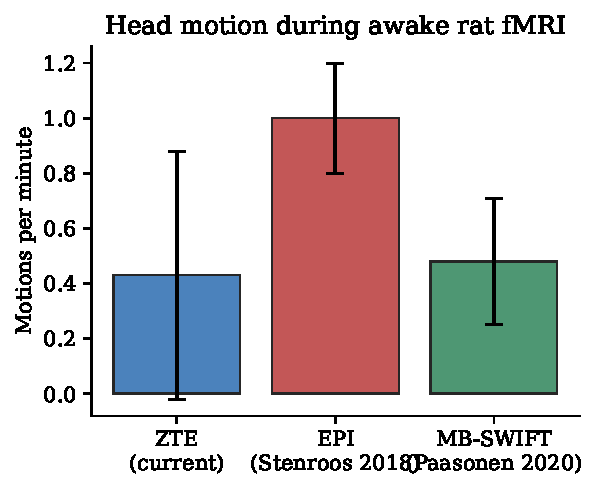
\includegraphics[width=0.70\linewidth]{figures/fig_motion.pdf}
  \caption{Head-motion occurrences per minute during awake rat fMRI for the current ZTE study, a previous EPI protocol using a comparable restraint holder \citep{stenroos2018}, and a previous quiet MB-SWIFT protocol \citep{paasonen2020}. Values are mean $\pm$ SD; ZTE $0.43 \pm 0.45$, EPI $1.0 \pm 0.20$, MB-SWIFT $0.48 \pm 0.23$ motions per minute.}
  \label{fig:motion}
\end{figure}

\begin{figure}[t]
  \centering
  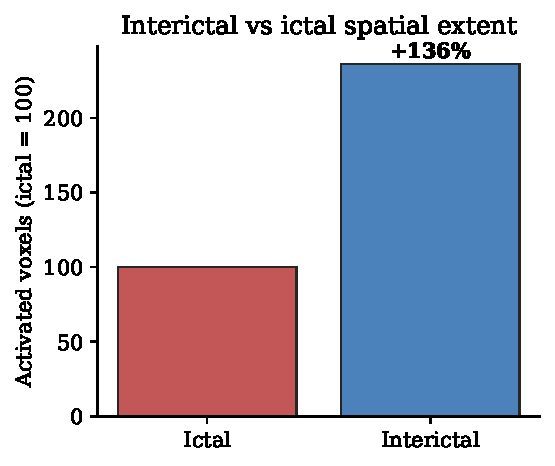
\includegraphics[width=0.70\linewidth]{figures/fig_voxels.pdf}
  \caption{Relative spatial extent of significantly responding voxels across the whole brain during interictal and ictal states. Interictal responses cover $136\%$ more voxels than ictal responses. Counts are normalized so that the ictal state equals 100.}
  \label{fig:voxels}
\end{figure}

\begin{figure}[t]
  \centering
  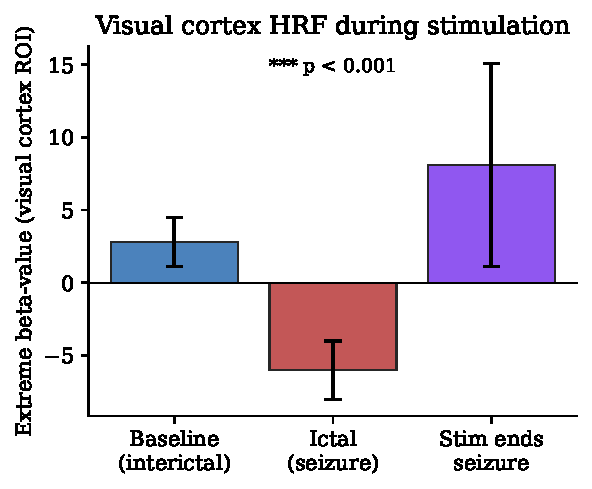
\includegraphics[width=0.70\linewidth]{figures/fig_beta_visual.pdf}
  \caption{Extreme beta-values of the hemodynamic response in the visual cortex ROI during (left) interictal baseline stimulation, (middle) stimulation that occurred during an ongoing seizure, and (right) stimulation that ended a seizure. Values are mean $\pm$ SD. All pairwise differences $p<0.001$.}
  \label{fig:betavisual}
\end{figure}

\begin{figure}[t]
  \centering
  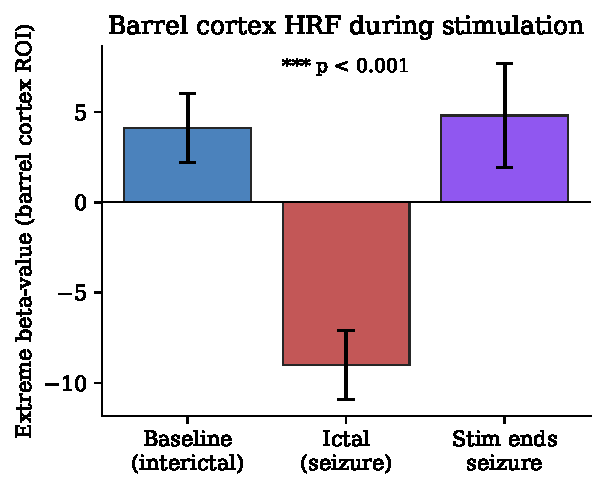
\includegraphics[width=0.70\linewidth]{figures/fig_beta_barrel.pdf}
  \caption{Extreme beta-values of the hemodynamic response in the barrel cortex ROI during (left) interictal baseline whisker stimulation, (middle) stimulation during an ongoing seizure, and (right) stimulation that ended a seizure. Values are mean $\pm$ SD. All pairwise differences $p<0.001$.}
  \label{fig:betabarrel}
\end{figure}
